\documentclass[conference]{IEEEtran}

\ifCLASSINFOpdf

\else

\fi


\usepackage{graphicx}

% correct bad hyphenation here
\hyphenation{op-tical net-works semi-conduc-tor}


\begin{document}

\title{The Creation of Competitive Co-evolution \\ by the Hands of God}



\author{\IEEEauthorblockN{Enrico Rotundo, Selene Beaz Santamaria, Andrea Borchelli Peperoni, Tommie Limberjack}
\IEEEauthorblockA{Vrije Universiteit Amsterdam \\
Amsterdam, Netherlands\\
Email: Enrico@smellLikePizza.italia}}



\maketitle


\begin{abstract}
In the context of robotics, intelligent behaviours are often achieved using neural networks as controllers evolved using  an evolutionary algorithm.
% */ not sure if this sentence is needed:
In the case of multiple individuals within a species, controllers can be either homogeneous or heterogeneous.
%maybe ommit /*
In this paper, we use competitive co-evolution of homo- and heterogeneous controllers in order to investigate its effects on the emergence of specialisation behaviour regarding a herding task.
% TODO: add what we have discovered
\end{abstract}


\IEEEpeerreviewmaketitle


\section{Introduction}
Evolutionary algorithms (EA) are biology inspired algorithms able to evolve entities over time through the generation, procreation and simulation of these entities. The entities subject to the evolution are referred to as individuals and the EA acts like the digital environment these individuals are born, live, procreate and die in.The evolution is usually controlled such that next generations improve along the runs.

In the field of robotics, EA's can be used to evolve the behavioural controller of a robot, these controllers are evolved as individuals in an EA.
Neural Networks (NN) are functions estimators or approximators nautal inspired by biological nervous systems, their design allows them to accept a high number of dimensional inputs. Neural Networks can be used to control the behaviour robots, where the inputs are come from the sensors making observations and the NN's weights are evolved by an evolutionary algorithm.

The complete evolutionary process can be run as a virtual simulation which exploits the current computer's computational power in order to evaluate many individuals in a reasonable time. Robotics employs both NNs and EAs in order to evolve intelligent behaviours that can pursue many given goals.

Tasks composition and complexity can vary based on the specific use case, in general it is subject of many studies aiming to solve different tasks.
For instance, tasks can be relatively small (e.g., moving objects) or more based on collaboration between a number of individuals.
Research investigates collective behaviour in order to asses to which extent collaboration between individuals is feasible.  

In this paper, we consider competitive co-evolution within a herding task which consists of a number of shepherds that herd a sheep into a corral.
Here we focus on evolving NNs as controllers for the agents.
Controllers can be assigned to agents with different approaches, the homogeneous approach uses the same controller for each type of agent (e.g., shepherds), meaning that each shepherd will be assigned the same controller. This one single controller is also the only evolved individual in the EA. In the heterogeneous approach each agent of a type gets their own controller and both controllers are separately evolved in the EA, using species.
% TODO are we going to talk about increasing complexity here?
Moreover, the task complexity can be increased by varying or introducing new agents like adding a fox.

We recap our objectives in the following list:

\begin{itemize}
	\item To compare homogeneity versus heterogeneity.
	\item To estimate the effect on homo versus heterogeneity of increasingly difficult task.
 	\item To develop controlled experiments through software simulations, using ad hoc Java libraries.
	\item To collect comprehensive results data.
\end{itemize}
 
\subsection{Research questions}
In the herding task, shepherds and sheep have opposing goals;
While the shepherds try to herd sheep into the corral, the sheep tries to escape through the left side of the pasture. Thus, species can be competitively co-evolved in a race to evolve strategies to accomplish opposing goals. Furthermore, the task complexity can be influenced by varying different parameters such as the number of present agents per each type or their relative movement speeds. Another type of dimension used to scale the difficulty is the type of controller used. Instances of different controller types are "passive", "active" and "intelligent". 

In this study an intelligent controller was added to the sheep, the intelligence of the controller is based on the assumption that since an artificial neural network is evolved, the sheep has the possibility to adapt to its environment through an evolutionary process. 
This process, in which many strategies are simulated and evaluated, is comparable to a learning process and enables adaptivity. 

Based on the assumption of intelligent sheep we state the following research questions:
 
\begin{enumerate}
	\item How does the competitive co-evolution affect the relation between homogeneous and heterogeneous (dog’s) controllers in a co-evolved herding task?
	\item How does increasing the difficulty (e.g.: by increasing the sheep’s speed) of a single task increase the necessity for heterogeneous controllers?
	\item How does increasing task complexity by adding more sheep affects the effectiveness of herding?
\end{enumerate}

\subsection{Hypothesis}
\label{sec:hypothesis}
The following hypothesis are in one to one relationship with the aforementioned research questions:

\begin{enumerate}
	\item Shepherds’ fitness in the heterogeneous case is overall higher than in the homogeneous case.
	\item Shepherds’ fitness in the heterogeneous case and sheep’s speed are inversely related, such that fitness decreases as speed increases.
	\item Shepherds’ fitness in the heterogeneous case and sheep’s multiplicity are inversely related, such that fitness decreases as speed increases.
\end{enumerate}

We now consider $H_1$, we leave the testing of the others as future work. The $H_0$, namely null hypothesis, is ``Shepherds’ fitness in the heterogeneous case is equivalent to the one of the homogeneous''.

\section{Literature}
 
\subsection{Coevolution}
It was as early as 1964 when Ehrlich and Raven focused their paper \cite{ehrlich1964butterflies} describing the effects of coevoultion in butterflies and plants.

In 1980 Janzen's \cite{janzen1980coevolution} formalised a clear definition for coevolution:
`` 'Coevolution' may be usefully defined as an evolutionary change in a trait of the individuals in one population in response to a trait of the individuals of a second population, followed by an evolutionary response by the second populations to the change in the first.''


\subsection{Competitive Coevolution}
Dawkins and Krebs described in their 1979 paper: ``Arms Races between and within Species'' \cite{dawkins1979arms}, the dynamics of, and created terminology for, competitive coevolution. Provided are examples of manifestations of competitive coevolution in natural systems.

In \cite{stanley2004competitive} Stanley and Miikkulainen showed that through the complexification of agent controllers in a competitive co-evolutionary setting, the controller's added complexity can be utilized through the generation of more advanced strategies as complexity increases.


\subsection{Homogeneity vs Heterogeneity in ANN's}
\cite{potter2001heterogeneity} performed a study to a tradeoff of homogeneity versus heterogeneity in the control systems of robots by allowing teams to coevolve their high-level controllers given different levels of difficulty of the task
Hypothesised was that: ``\textit{simply increasing the difficulty of a task is not enough to induce a team of robots to create specialists.}''
Task difficulty was varied by replacing one adversary's passive controller with an active variant supposedly proving that increased difficulty did not justify the use of heterogeneous controllers.
However, increased difficulty was never implemented structurally nor tested methodologically. 



\section{Model}
Our model is based on Potter et al. work \cite{potter2001heterogeneity}. The task domain relates to a herding task that simulates shepherd robots trying to push sheep robots into a corral. The environment consists of a 37 x 37 foot pasture with fences on the top and bottom; the corral is positioned on the right side, and the pasture is open on the left side for the sheep to escape.

We module the task complexity by controlling the number of agents of each type that take part in the task. Thus, we operationalize it as the sheep to dog ratio, with increased ratio implying a more complex task for the shepherds. 

We compute the center of sheep - which is equal to the position of the sheep when there is only one - and take is as center for a polar coordinate system. Therefore, the first component for a coordinate is the distance to the center, called the range. A line is created between this center and the midpoint for the entrance of the corral, from which angles are created for the second component of the polar coordinates, called bearings. 


\subsection{NN design}
The controllers for the agents are composed of neural networks, with each agent containing a multiplayer perceptron, with one hidden layer. The inputs for the networks come in pairs as the range and bearing of other agents in the polar coordinate system previously described. In a simple network, where an agent can only see one other agent, the network consists of two input nodes and a bias, and its hidden layer has three nodes. Alternatively, if the agent can see two other agents it has a more complex neural network, with four input nodes and a bias, and five nodes in its hidden layer. 

\subsection{Evolution of NN controllers}
The algorithm used to evolve the controllers follows the frameworks of evolutionary strategies. The genome is an array of doubles consisting of the weights for the neural network: 17 for a simple network and 37 for a complex network.

Mu has a value of 10 and lambda a value of 10. 
Tournament selection, tournament size is 5
All controllers are evaluated through 10 trials of the task and the average is taken as fitness function. 

Fitness for shepherd is the distance from every sheep to the corral. The range is [-X, 0]

Fitness for sheep is the distance from every sheep to the corral. The range is [0, +X]

Both are maximization problems.


\subsection{Shepherds controllers}
Input is information about self and the closest shepherd. We assume the shepherds need to evolve cooperation behaviours, and thus need information about the other shepherds around. However, in an attempt to be realistic and keep the network complexity low, we only provide the controller with information for the closest shepherd. 

\subsection{Sheep controllers}
Input is information about closest shepherd and closest sheep. This time we assume sheep aim for both competitive behaviour against the shepherds and cooperative behaviour with other sheep. In order to avoid the shepherd and be able to escape, sheep must have information about the closest shepherd; but they also have a strong preference to stay in group and so need information about the closes sheep around them. 

\section{Implementation}
We use mason, with ECJ for the evolutionary process. We use neuroph as the library for neural networks. 

Both types of agents have obstacle avoidance built into their behaviour. Shepherds avoid bumping into fences, the corral or other agents within a 3 simulation unit ratio. Meanwhile, the sheep can only avoid fences and other agents within a 2 simulation unit ratio. 

\section{Experiment}
\label{sec:experiment}
In this section we detail the design of the experiments performed in this paper. In order to test our hypothesis, we perform coevolution across 100 generations. We run the simulation 40 times and perform statistical analysis to get 95\% confidence intervals.


We first consider the experiments that relate to $H_1$ listed in ~\ref{sec:hypothesis}. To investigate the difference between homogeneous and heterogeneous controllers for the shepherd agents, we first explore a scenario with two shepherd and one sheep. 
\begin{itemize}
	\item 2 homogeneous shepherd’s vs 1 (intelligent) sheep
	\item 2 heterogeneous shepherd’s vs 1 (intelligent) sheep
\end{itemize}
 
 Later on, we compare different scenarios with different number of dogs corralling one sheep. This way the task complexity varies by having different sheep to dog ratios. 



\section{Results}
In this section we present the results of the experiment detailed in Section ~\ref{sec:experiment}.

\begin{figure}[ht]
\centering
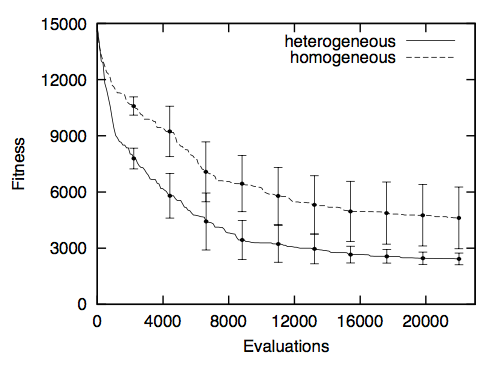
\includegraphics[width=3.3in]{imgs/homo_vs_hetero.png}
\caption{TODO.}
\label{fig:homo_vs_hetero}
\end{figure}

\section{Conclusion}
The conclusion goes here.

\subsection{Future work}
TODO

-In a competitive co-evolution, how does increasing task complexity by adding more sheep affects the effectiveness of herding? %TODO: fix

-[In a competitive co-evolution, do heterogeneous sheep perform better than homogeneous?] %TODO: fix



\bibliographystyle{abbrv}
\bibliography{bibliography}



\end{document}

